\documentclass[a4paper]{article}

\usepackage[T1]{fontenc}
\usepackage[utf8]{inputenc}
\usepackage{lmodern}

\usepackage[english]{babel}
\usepackage{csquotes}

\usepackage[notes,backend=biber]{biblatex-chicago}

\usepackage{graphicx}
\usepackage{float}

\bibliography{sample}

\begin{document}
\title{LietoMe: Emotional parameter based Telepathy through brain-computer interface}
\author{Tongda Xu}
\maketitle

\section{Abstract}

\begin{figure}[H]
	\centering
	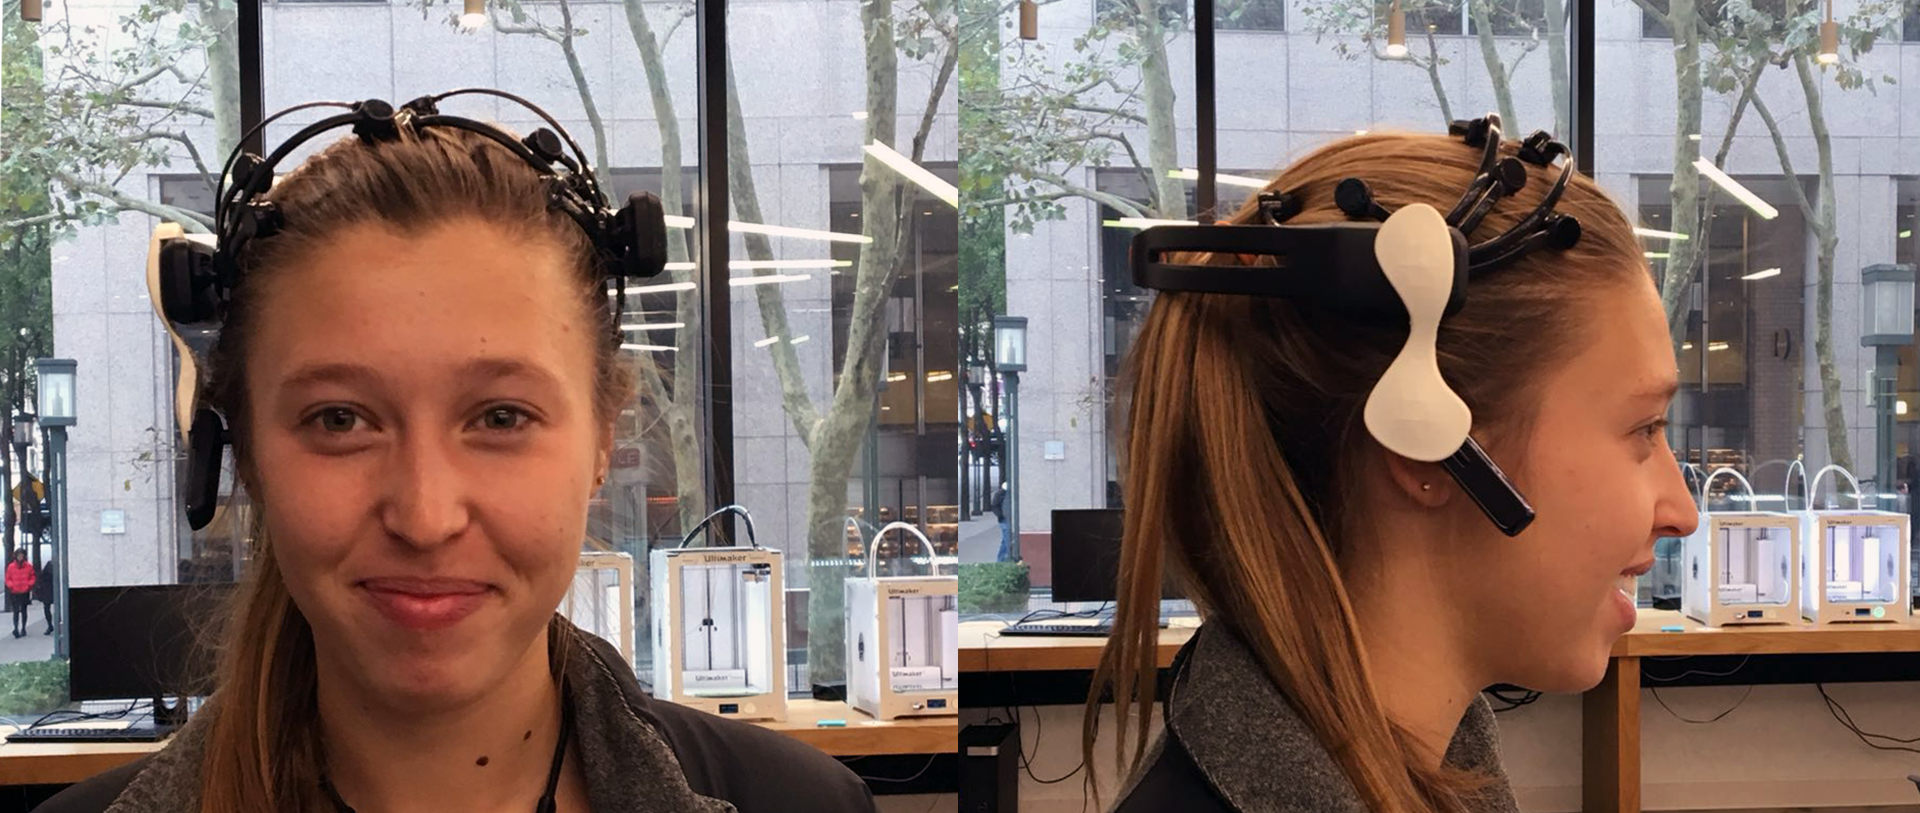
\includegraphics[width=\linewidth]{Diagram_1}
	\caption{The LietoMe Prototype with Reader and Sender}
	\label{fig:prototype}
\end{figure}

This paper describe LietoMe, a emotional parameter based Telepathy prototype. LietoMe adopts brain-computer interface to read the emotional state of user, sharing it through UDP server and finally converted into sound signals received other nearby users.

Aimed to help people express feeling, LietoMe reads and share users' feeling implicitly and involuntarily. The users could not choose not to send her mind state nor not receiving others. It could be interpreted as a device from one of future dystopia where everyone has no secret feelings.

\section{Introduction}

Coined in 1882 by poet Frederic Myers, telepathy is initially defined as \textit {forms of occult relation or communication between people at distance}. \autocite{luckhurst2002invention} Historically, it is a heated topic strongly connected with Gothic imagination, woman's hyper-sensitivity and psycho-analysis \autocite{freud1955dreams}.

Recent scholars and technician pick the concept up as a mean of augmented communication to modify speech or texting. \textit{Project Telepathy} in 2018 presents an Electromyography(EMG) based silent speech recognition and broadcasting system allowing the enhancement the privacy and effective size of public speech \autocite{bourland2017project}. 

Similarly, LietoMe aims to solve the emotion expression issue for those with difficulty. Modern psychologists argue that expression of emotion serves as a crucial element in adaptation, including communicating and regulating internal states, developing and maintaining social interactions \autocite{bonanno2004importance}. LietoMe provides a emotional communication pathway circumvents of personal willingness, which might hinder a necessary emotion expression.

\section{Design Consideration and Implement}

\begin{figure}[H]
	\centering
	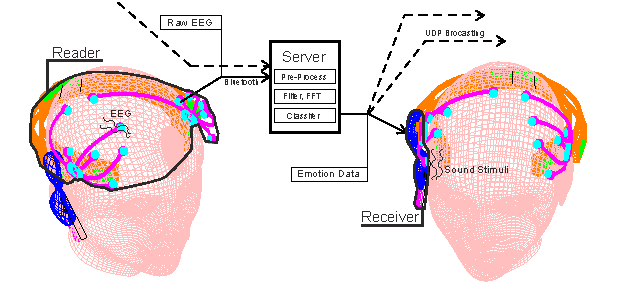
\includegraphics[width=\linewidth]{Diagram_2}
	\caption{The Composition and data flow of LietoMe}
	\label{fig:comp}
\end{figure}

The LietoMe system is composed of 3 parts:

\begin{itemize}
    \item \textbf {Reader}: The hardware of mind reader is an Emotiv Epoch 16-Channel EEG headset. It captures the raw EEG data at 240HZ and sends raw EEG to \textbf{Server} by Bluetooth.
    \item \textbf {Server}: The server is a Thinkpad X1 Carbon with Win 10 Pro running the software. The software would first filter the data, remove artifacts such as eye movement or acceleration \autocite{le2011method}. Then the cleaned data would go through Fast Fourier Transformation mapping into band power. The band power would be send to a Support Vector Machine (SVM) based emotion classifier. For each class, a score would be scaled to 0-100. The emotion with highest score (probability) would be passed through Speech Synthesis and send to the \textbf{Receiver}.
    \item \textbf{Receiver}: The actuator is as simple as a wireless earpod receiving the synthesized sound from \textbf {Server} and play the sound to people wearing it.
\end{itemize}

When wore and connected to the Server, the device would iterative send EEG data to the server. The server would estimate the distance between users by Bluetooth signal strength. When two users are close enough, the server would send the synthesized sound containing her emotion state description to each other iterative.

In this way, the emotion condition could be shared between people involuntarily.

\section{Conclusion and Discussion}

This paper presents LietoMe, a emotional parameter based Telepathy system aims to a better share of feeling between people. 

A major problem of prototype implement is that only one Emotiv EEG headset could be afford by author (Sponsor me Sir! I can do better!). The prototype losses 50 \% of convincing without a multi-user experiment.

Another problem the over-expression issue. Research also reveal that over-expression of emotion could cause problem \autocite{bonanno2004importance}. Despite LietoMe could distinguish negative emotion with positive emotion, it could not judge the context to express them properly.


\printbibliography

\end{document}